\question In the figure below, the gray sphere has a radius $R=14$ cm and is positioned with its center at the origin. The gray sphere is a conductor and is in equilibrium. In this problem, the origin of the coordinate system is the center of the sphere and the $x$ and $y$ directions are depicted in the diagram.

\begin{center}
	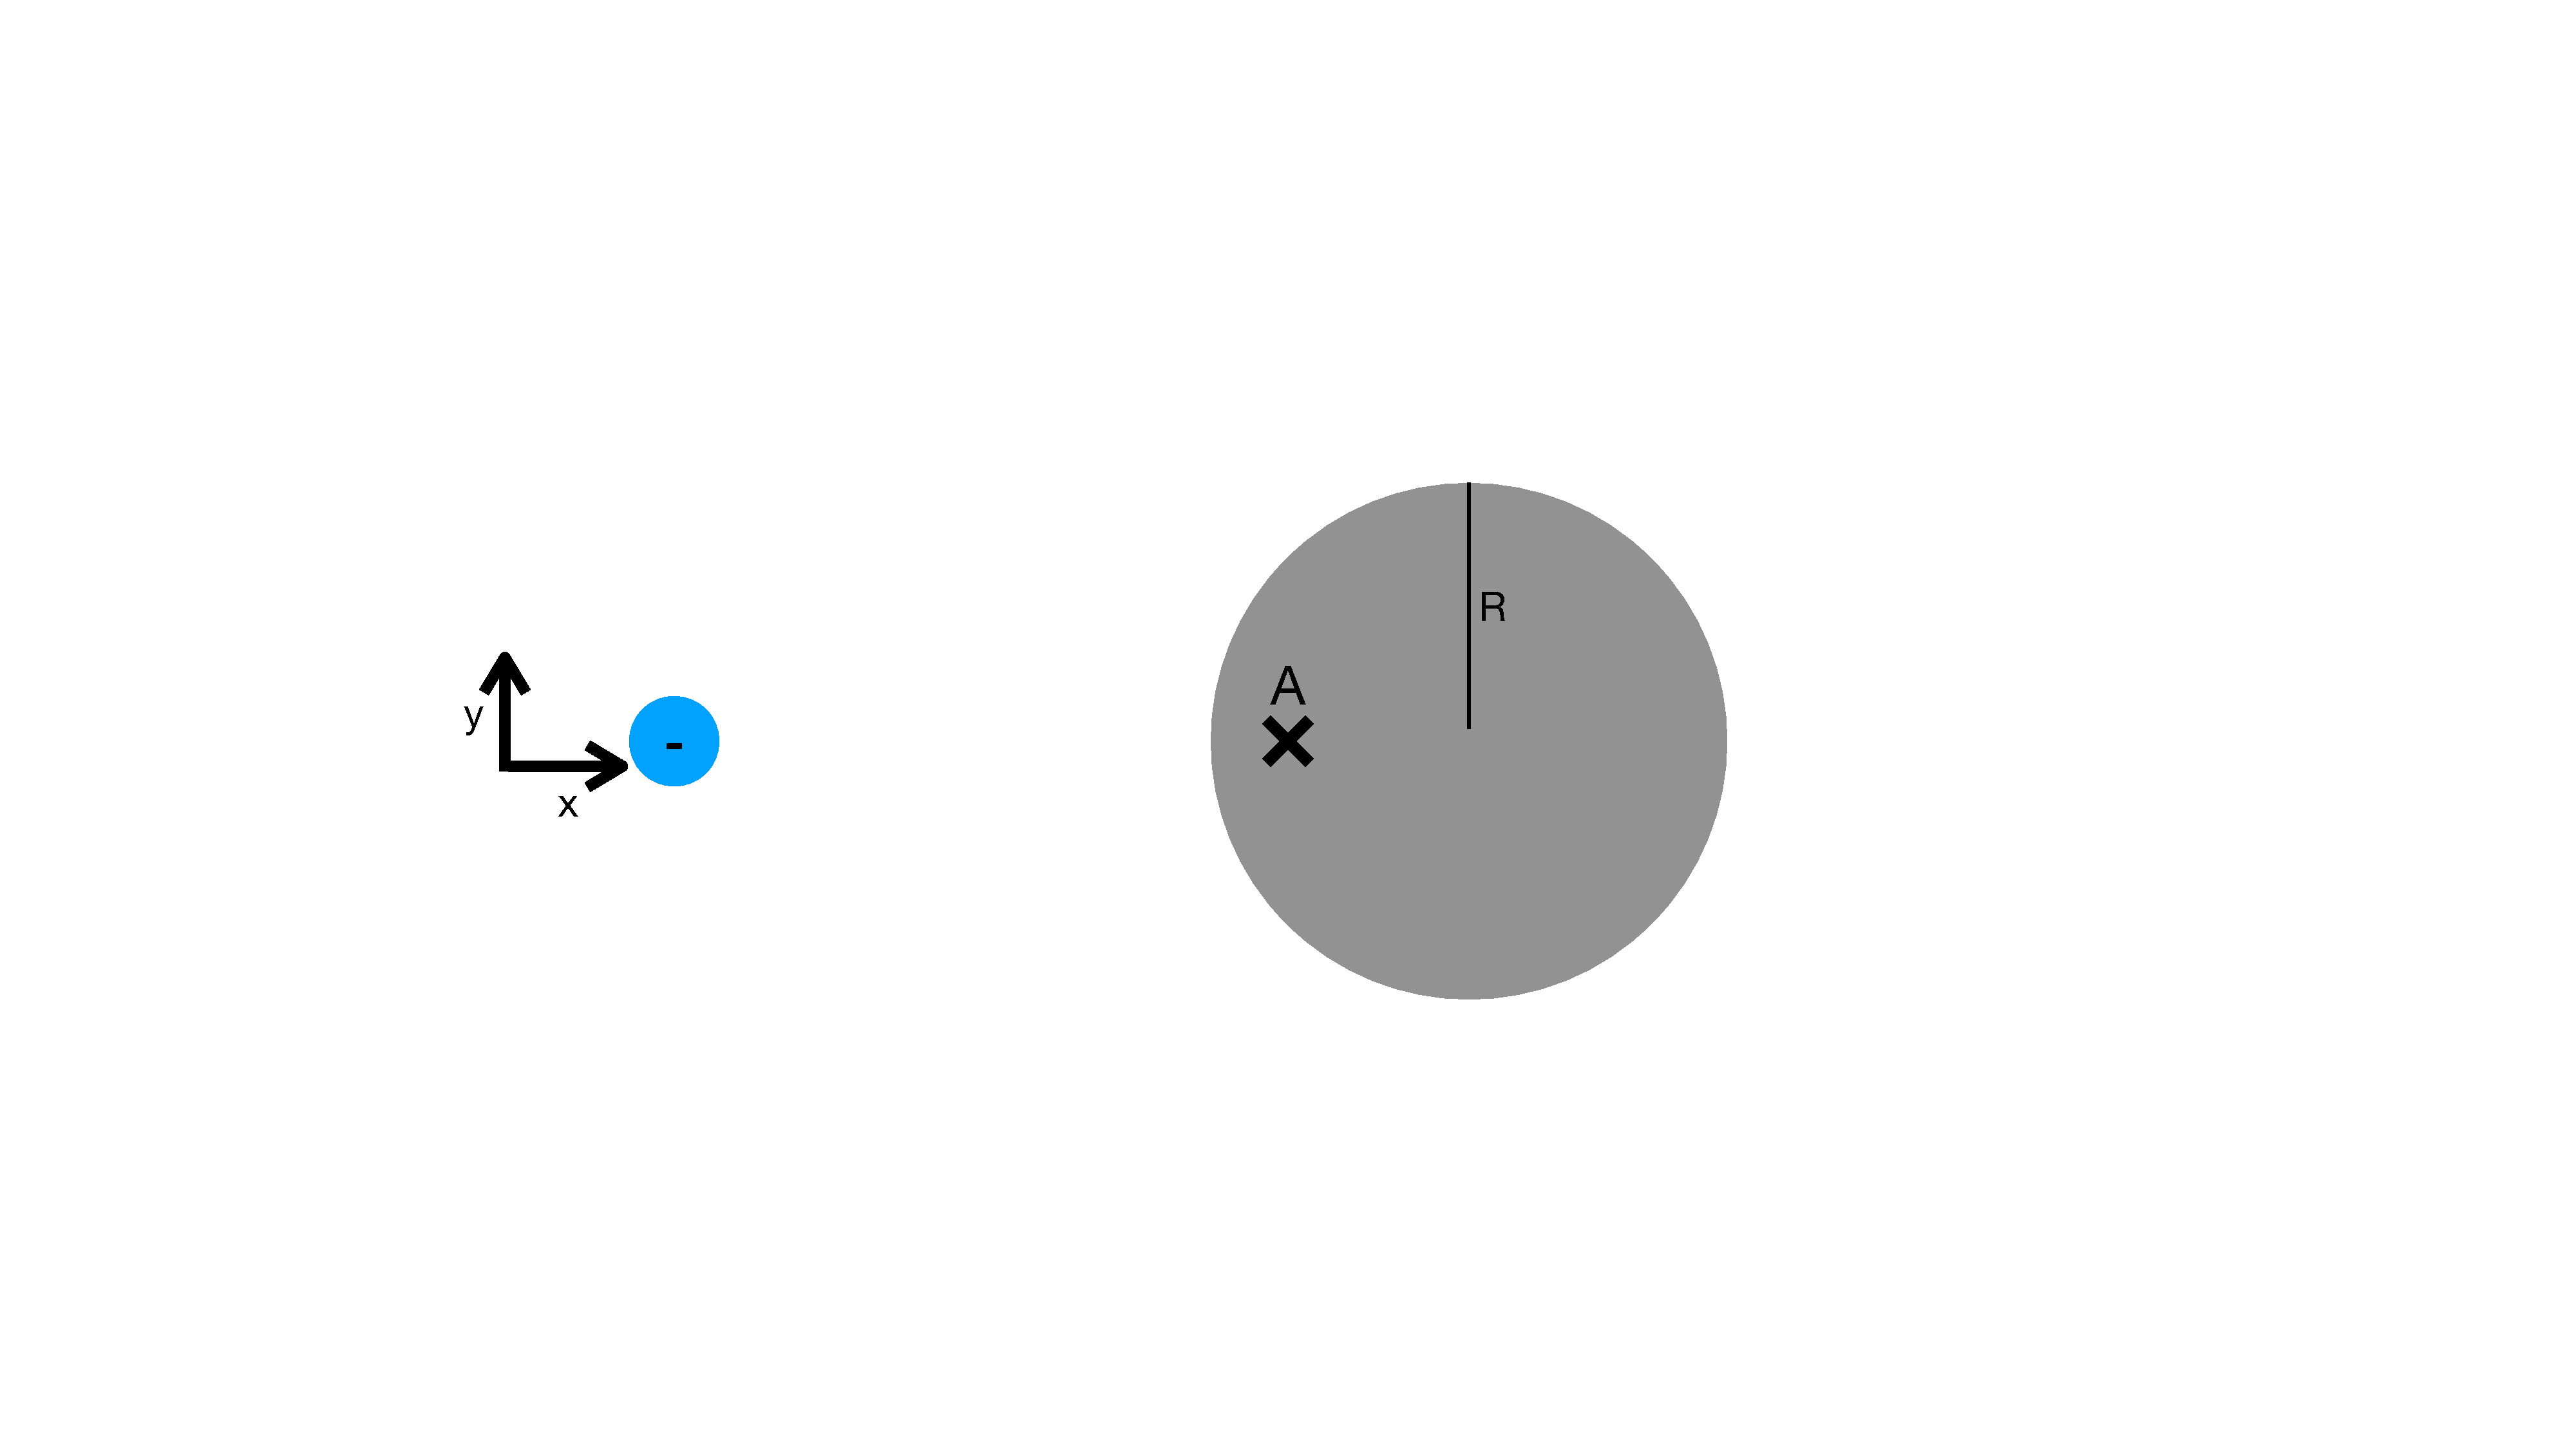
\includegraphics[width=.5\textwidth]{p4diag1}
\end{center}

\begin{parts}
	\part A negative point charge $q=-12$ nC is brought near the conducting sphere and placed at the position $\vec{r}_\mathrm{chg}=<-26,0,0>$ cm. What is the net electric field $\vec{E}_\mathrm{net}$ at the position $A$ (the position of $A$ is given by $\vec{r}_A=<-12,0,0>$  cm)?
	\vspace{5cm}
	\part What is the induced field $\vec{E}_\mathrm{ind}$, the electric field produced by the polarized charges in the conductor, at point $A$?
\end{parts}